% !TeX program = xelatex
% 编译：xelatex 01-信号的自变量变换.tex（VS Code 的 LaTeX Workshop 会读上一行，自动用 xelatex）
% 来源：2022 浙江大学《信号与系统》胡浩基老师，第 1 章 §1.4.2「信号的自变量变换」一节课（视频约 44 分钟）。
\documentclass[UTF8,a4paper,11pt]{ctexart}
\usepackage{amsmath,amssymb}
\usepackage{geometry}
\geometry{margin=2.4cm}
\usepackage{xcolor}
\usepackage{mdframed}
\usepackage{booktabs}
\usepackage{enumitem}
\usepackage{tikz}
\usepackage{float}

\setCJKmainfont{Songti SC}[BoldFont={Songti SC Bold}]
\setCJKsansfont{PingFang SC}

\newmdenv[backgroundcolor=blue!4,linecolor=blue!50!black,linewidth=1pt,innertopmargin=6pt,innerbottommargin=6pt]{rememberbox}
\newenvironment{remember}{\begin{rememberbox}\textbf{必须背下来}\par\smallskip}{\end{rememberbox}}
\newmdenv[backgroundcolor=yellow!8,linecolor=orange!70!black,linewidth=1pt,innertopmargin=6pt,innerbottommargin=6pt]{notebox}
\newenvironment{note}{\begin{notebox}\textbf{说明}\par\smallskip}{\end{notebox}}
\newcommand{\Sa}{\operatorname{Sa}}
\renewcommand{\d}{\,\mathrm{d}}

% ---------------------------------------------------------------- 画图用的小宏
% 三角形：左端 a、峰在 b（高 1）、右端 c。#1 横向比例，#2 标题，#6 刻度列表
\newcommand{\tripanel}[6]{%
\begin{tikzpicture}[x=#1,y=1.1cm,>=stealth]
  \draw[->] (-8,0) -- (8.6,0) node[right,font=\scriptsize] {$t$};
  \draw[->] (0,-0.2) -- (0,1.4);
  \draw[very thick,blue!70!black] (#3,0) -- (#4,1) -- (#5,0);
  \draw[dotted,gray] (#4,0) -- (#4,1);
  \foreach \k in {#6} { \draw (\k,0.05) -- (\k,-0.05) node[below,font=\scriptsize] {$\k$}; }
  \node[font=\scriptsize,anchor=south] at (0,1.45) {#2};
\end{tikzpicture}}
% 直角三角形：在 p0 处竖直边（高 2），斜边落到 p1。#1 横向比例
\newcommand{\rtpanel}[5]{%
\begin{tikzpicture}[x=#1,y=0.65cm,>=stealth]
  \draw[->] (-5,0) -- (6.2,0) node[right,font=\scriptsize] {$t$};
  \draw[->] (0,-0.3) -- (0,2.8);
  \draw[very thick,blue!70!black] (#3,0) -- (#3,2) -- (#4,0);
  \node[left,font=\scriptsize] at (0,2) {$2$};
  \foreach \k in {#5} { \draw (\k,0.1) -- (\k,-0.1) node[below,font=\scriptsize] {$\k$}; }
  \node[font=\scriptsize,anchor=south] at (0,2.95) {#2};
\end{tikzpicture}}
% 离散火柴杆
\newcommand{\stem}[2]{\draw[thick,blue!70!black] (#1,0) -- (#1,#2); \fill[blue!70!black] (#1,#2) circle (1.8pt);}
\newcommand{\stemzero}[1]{\fill[blue!70!black] (#1,0) circle (1.4pt);}

\title{信号的自变量变换\\\large 浙江大学 2022《信号与系统》（胡浩基）§1.4.2 听课笔记}
\author{}
\date{}

\begin{document}
\maketitle

\begin{note}
这份笔记由视频整理而来，来源要分清：
\begin{itemize}[nosep]
\item 老师的口述：来自语音转写。这次直接用 whisper 的 large-v3-turbo 模型（关闭上下文复用、加了术语提示词）转写，没有出现复读，错字很少；
\item 题目里的图和数字：来自画面（PPT 与黑板截图）。个别题目的口述与画面不一致时，以画面为准（见 \S3.3）；
\item 标注「（补充）」的内容是我自己加的，课上没讲，或我没有核对书。
\end{itemize}
\end{note}

%==================================================================
\section{一句话主干}
\textbf{自变量变换}(transformation of the independent variable)：把信号 $x(t)$ 的「$t$」换成「$at+b$」，得到新信号 $x(at+b)$。从图像上看，就是把波形沿横轴\textbf{平移}、\textbf{翻转}、\textbf{压缩或拉伸}，纵轴的值不变。

老师这节课的做法很特别：书上（第 23 页，1.4.2）讲得比较抽象，所以他\textbf{用做题的方式来讲}，并给出\textbf{四句口诀}。这四句口诀是本节要背的核心。

%==================================================================
\section{四句口诀}

\begin{remember}
做这类题目的口诀（课件原文）：
\begin{enumerate}[nosep]
\item \textbf{化成标准形式}。
\item \textbf{前有负号翻转}。
\item \textbf{系数大于 $1$ 压缩，系数小于 $1$ 拉伸}（指系数的\textbf{绝对值}）。
\item \textbf{加号左移，减号右移}。
\end{enumerate}
\end{remember}

\subsection{例 1：三角波的 $x(3t+6)$ 与 $x(-3t+6)$}
题目：已知 $x(t)$ 是下面的三角波：$t\in[0,3]$ 上升、$t\in[3,6]$ 下降，最高点高度为 $1$。画出 $x(3t+6)$ 和 $x(-3t+6)$。老师说这是「高中的知识，只是做得快慢的问题」。

\begin{figure}[H]
\centering
\tripanel{0.42cm}{$x(t)$}{0}{3}{6}{0,3,6}
\caption{已知的三角波 $x(t)$：在 $t=0$ 处为 $0$，$t=3$ 处升到 $1$，$t=6$ 处回到 $0$。}
\end{figure}

\subsubsection*{方法一：固定关键点（老师先讲的，好理解）}
把波形上的三个关键点（$t=0,3,6$）固定下来，问：在新信号里，这三个点分别跑到了哪里？思路是：新信号 $x(3t+6)$ 在 $t$ 处的值，等于 $x$ 在「括号里那个数」处的值。所以让括号里的数等于原来的关键点：
\begin{center}
\begin{tabular}{@{}cccc@{}}
\toprule
原来的关键点 & $x(\cdot)$ 的值 & 令 $3t+6$ 等于它 & 新信号里对应的 $t$\\
\midrule
$0$ & $0$ & $3t+6=0$ & $t=-2$\\
$3$ & $1$（峰）& $3t+6=3$ & $t=-1$\\
$6$ & $0$ & $3t+6=6$ & $t=0$\\
\bottomrule
\end{tabular}
\end{center}
所以 $x(3t+6)$ 是一个三角波：在 $t=-2$ 处为 $0$，$t=-1$ 处是峰（高 $1$），$t=0$ 处回到 $0$。

同样 $x(-3t+6)$：$-3t+6=0\Rightarrow t=2$；$=3\Rightarrow t=1$；$=6\Rightarrow t=0$。它是 $t=0$ 处为 $0$、$t=1$ 处是峰、$t=2$ 处回到 $0$ 的三角波。

老师说这种方法他\textbf{不是不推荐}，但希望大家牢牢记住下面的口诀，因为到后面你脑子里应该有一幅图：信号「移来移去、翻转过来翻转过去、拉伸缩短」。

\subsubsection*{方法二：四步口诀}
\textbf{$x(3t+6)$}：
\begin{enumerate}[nosep]
\item \textbf{化成标准形式}：把 $t$ 前面的系数提出来，$x(3t+6)=x\bigl(3(t+2)\bigr)$；
\item \textbf{前有负号翻转}：$3$ 前面没有负号，这步可以不做；
\item \textbf{系数大于 $1$ 压缩}：系数是 $3>1$，横向压缩 $3$ 倍。$x(t)$ 的关键点 $0,3,6$ 除以 $3$，变成 $0,1,2$；
\item \textbf{加号左移}：括号里是 $t+2$，是加号，左移 $2$ 个单位：$0,1,2$ 变成 $-2,-1,0$。
\end{enumerate}

\textbf{$x(-3t+6)$}：
\begin{enumerate}[nosep]
\item \textbf{化成标准形式}：$x(-3t+6)=x\bigl(-3(t-2)\bigr)$。（验算：$-3\times(-2)=6$。）
\item \textbf{前有负号翻转}：先画 $x(-t)$，以纵轴为对称轴翻过去：关键点 $0,3,6$ 变成 $0,-3,-6$；
\item \textbf{系数绝对值 $3>1$ 压缩}：针对翻转后的图压缩 $3$ 倍：$-6,-3,0$ 变成 $-2,-1,0$，得到 $x(-3t)$；
\item \textbf{减号右移}：括号里是 $t-2$，是减号，右移 $2$ 个单位：$-2,-1,0$ 变成 $0,1,2$。
\end{enumerate}
最后得到的答案和方法一的结果一致（峰在 $t=1$，两端在 $t=0$ 和 $t=2$）。

\begin{figure}[H]
\centering
\begin{minipage}{0.48\textwidth}\centering
\tripanel{0.4cm}{$x(t)$}{0}{3}{6}{0,3,6}
\end{minipage}
\begin{minipage}{0.48\textwidth}\centering
\tripanel{0.4cm}{$x(3t)$：压缩 3 倍}{0}{1}{2}{0,1,2}
\end{minipage}

\medskip
\tripanel{0.4cm}{$x(3t+6)=x(3(t+2))$：左移 2}{-2}{-1}{0}{-2,-1,0}
\caption{$x(3t+6)$ 的做法：先压缩（$x(3t)$），再左移 $2$。}
\end{figure}

\begin{figure}[H]
\centering
\begin{minipage}{0.48\textwidth}\centering
\tripanel{0.4cm}{\textcircled{1} $x(t)$}{0}{3}{6}{0,3,6}
\end{minipage}
\begin{minipage}{0.48\textwidth}\centering
\tripanel{0.4cm}{\textcircled{2} $x(-t)$：翻转}{-6}{-3}{0}{-6,-3,0}
\end{minipage}

\medskip
\begin{minipage}{0.48\textwidth}\centering
\tripanel{0.4cm}{\textcircled{3} $x(-3t)$：压缩 3 倍}{-2}{-1}{0}{-2,-1,0}
\end{minipage}
\begin{minipage}{0.48\textwidth}\centering
\tripanel{0.4cm}{\textcircled{4} $x(-3t+6)=x(-3(t-2))$：右移 2}{0}{1}{2}{0,1,2}
\end{minipage}
\caption{$x(-3t+6)$ 的四步：\textcircled{1}$\to$\textcircled{2} 翻转，\textcircled{2}$\to$\textcircled{3} 压缩，\textcircled{3}$\to$\textcircled{4} 右移。}
\end{figure}

老师说：这四步希望大家牢牢掌握。

\subsection{为什么口诀成立（补充）}
老师说「大家是高考的能手，自己想一想应该能知道道理」，没有展开。这里把道理写出来，初学者记住这三条就不容易错。\emph{（以下是我（补充）的，没有核对书。）}

\begin{enumerate}
\item \textbf{为什么要化成 $x(a(t+b/a))$（提出系数）}：因为「平移」平移的是 $t$ 本身。$x(3t+6)$ 里的 $6$ 是对 $3t$ 加的，不是对 $t$ 加的，所以真正平移的距离是 $6/3=2$，不是 $6$。化成标准形式 $x(3(t+2))$ 之后，括号里的 $2$ 才是直接作用在 $t$ 上的平移量。
\item \textbf{为什么加号左移}：新信号在 $t$ 处的值，是原信号在 $t+2$ 处的值。原信号在 $p$ 处的特征（比如峰），在新信号里要到 $t+2=p$，即 $t=p-2$ 处才看得到，比原来位置\textbf{小}，就是向左。减号反之。
\item \textbf{为什么系数大于 $1$ 压缩}：$x(3t)$ 在 $t$ 处的值是原信号在 $3t$ 处的值，原信号走完 $3$ 个单位，新信号只用 $1$ 个单位，所以「变快」了，波形被挤窄。系数小于 $1$ 则相反，被拉宽。
\end{enumerate}

\begin{note}
一个容易踩的坑（补充）：先化成标准形式，再按「翻转 $\to$ 压缩或拉伸 $\to$ 平移」的顺序做，平移量是 $b/a$，不是 $b$。如果坚持先平移再压缩，平移量就是 $b$（即 $x(t+6)$，再压缩 $3$ 倍），结果相同，但很容易搞错，所以老师把「先化成标准形式」放在第一条。
\end{note}

\subsection{例 2：$x\bigl(-\tfrac12t+1\bigr)$}
这是老师抽同学上来做的第二道题。\textbf{注意}：转写里把它听成了「$x(-2t+1)$」，但 PPT 上写的是 $x\bigl(-\tfrac12t+1\bigr)$（画面里能看到分数 $\tfrac12$），所以以画面为准。

已知 $x(t)$ 是一个直角三角形：在 $t=-1$ 处有一条竖直边（高 $2$），斜边向右下落到 $t=0$ 处的 $0$。老师说那位同学的答案和他的完全一样（课堂上没有读出具体数值）。下面是我按四步口诀算出来的：
\begin{enumerate}[nosep]
\item 标准形式：$x\bigl(-\tfrac12t+1\bigr)=x\bigl(-\tfrac12(t-2)\bigr)$；
\item 前有负号翻转：竖直边从 $t=-1$ 翻到 $t=1$，斜边落点仍在 $0$；
\item 系数绝对值 $\tfrac12<1$ 拉伸：横向拉伸 $2$ 倍，竖直边到 $t=2$，落点仍是 $0$；
\item 减号右移 $2$：竖直边到 $t=4$，落点到 $t=2$。
\end{enumerate}
\emph{（我自己验算了两点：$t=4$ 时 $x(-\tfrac12\cdot4+1)=x(-1)=2$；$t=2$ 时 $x(0)=0$。）}

\begin{figure}[H]
\centering
\begin{minipage}{0.48\textwidth}\centering
\rtpanel{0.4cm}{\textcircled{1} $x(t)$}{-1}{0}{-1,0}
\end{minipage}
\begin{minipage}{0.48\textwidth}\centering
\rtpanel{0.4cm}{\textcircled{2} $x(-t)$：翻转}{1}{0}{0,1}
\end{minipage}

\medskip
\begin{minipage}{0.48\textwidth}\centering
\rtpanel{0.4cm}{\textcircled{3} $x(-\frac t2)$：拉伸 2 倍}{2}{0}{0,2}
\end{minipage}
\begin{minipage}{0.48\textwidth}\centering
\rtpanel{0.4cm}{\textcircled{4} $x(-\frac t2+1)$：右移 2}{4}{2}{2,4}
\end{minipage}
\caption{$x(-\frac12t+1)$ 的四步。}
\end{figure}

\subsection{例 3：反过来做——已知 $x(3-2t)$，求 $x(t)$}
这道题「反过来了」：给的是变换\emph{之后}的波形，要画\emph{原来}的 $x(t)$。老师说你知道套路就不难。

题目给的 $x(3-2t)$ 的波形（PPT 上）：$t\in[2,3]$ 上高度 $1$，$t\in[3,4]$ 上高度 $2$，其余为 $0$。

\textbf{老师的思路：变量代换。}设 $u=3-2t$，则 $t=\dfrac{3-u}{2}$。已知的是「关于 $t$ 的函数 $x(3-2t)$」，把它的图像当成一个已知函数 $g$，则要求的 $x(t)=g\bigl(\tfrac{3-t}{2}\bigr)$，也就是 $g$ 做了自变量变换。把它化成标准形式：
\[
g\Bigl(\frac{3-t}{2}\Bigr)=g\Bigl(-\frac12\,(t-3)\Bigr),
\]
然后照口诀：
\begin{enumerate}[nosep]
\item 标准形式：$-\tfrac12(t-3)$；
\item 前有负号翻转：$g$ 的图（在 $[2,4]$）翻成 $[-4,-2]$；
\item 系数绝对值 $\tfrac12<1$ 拉伸 $2$ 倍：$[-8,-4]$；
\item 减号右移 $3$：$[-5,-1]$。
\end{enumerate}
答案：$x(t)$ 在 $[-5,-3]$ 上高度 $2$，在 $[-3,-1]$ 上高度 $1$。

\begin{figure}[H]
\centering
\begin{minipage}{0.48\textwidth}\centering
\begin{tikzpicture}[x=0.55cm,y=0.7cm,>=stealth]
  \draw[->] (-1,0) -- (5.6,0) node[right,font=\scriptsize] {$t$};
  \draw[->] (0,-0.3) -- (0,2.8);
  \draw[very thick,blue!70!black] (2,0) -- (2,1) -- (3,1) -- (3,2) -- (4,2) -- (4,0);
  \node[left,font=\scriptsize] at (0,1) {$1$};
  \node[left,font=\scriptsize] at (0,2) {$2$};
  \foreach \k in {1,2,3,4} { \draw (\k,0.08) -- (\k,-0.08) node[below,font=\scriptsize] {$\k$}; }
  \node[font=\scriptsize,anchor=south] at (2.5,2.9) {已知：$x(3-2t)$};
\end{tikzpicture}
\end{minipage}
\begin{minipage}{0.48\textwidth}\centering
\begin{tikzpicture}[x=0.5cm,y=0.7cm,>=stealth]
  \draw[->] (-6.5,0) -- (2,0) node[right,font=\scriptsize] {$t$};
  \draw[->] (0,-0.3) -- (0,2.8);
  \draw[very thick,blue!70!black] (-5,0) -- (-5,2) -- (-3,2) -- (-3,1) -- (-1,1) -- (-1,0);
  \node[right,font=\scriptsize] at (0,1) {$1$};
  \node[right,font=\scriptsize] at (0,2) {$2$};
  \foreach \k in {-5,-3,-1} { \draw (\k,0.08) -- (\k,-0.08) node[below,font=\scriptsize] {$\k$}; }
  \node[font=\scriptsize,anchor=south] at (-3,2.9) {所求：$x(t)$};
\end{tikzpicture}
\end{minipage}
\caption{左：已知的 $x(3-2t)$；右：所求的 $x(t)$。（左图的数据来自 PPT，右图来自黑板上老师的最终答案。）}
\end{figure}

\paragraph{课堂上的讲评。}这道题老师请一位同学上黑板做，同时自己在旁边按口诀逐步讲：翻转后区间变成 $[-4,-2]$，拉伸 $2$ 倍后坐标都乘 $2$，变成 $[-8,-4]$，最后「减号要右移」。老师对这位同学的评语是「基本上是对的」，但指出两个习惯：一是不要把几个图画在同一根坐标轴上，容易自己分不清；二是要在图上标注 $t$ 和关键点的数值，「要细心一点」。\emph{（我最初把这段理解成同学漏了右移，重新对照转写后发现不是，已更正。）}

\emph{（补充，用上面的变换验算：$x(t)=g\bigl(\tfrac{3-t}{2}\bigr)$。取 $t=-4$：$\tfrac{3-(-4)}{2}=3.5\in[3,4]$，$g=2$；取 $t=-2$：$\tfrac{3-(-2)}{2}=2.5\in[2,3]$，$g=1$。与答案一致。）}

\paragraph{书上的练习。}老师说书上第 31 页的习题 1-7 和 1-8 都是这类题，也都布置给了大家，回去自己练习。

%==================================================================
\section{离散信号的自变量变换}
口诀仍然是这四句，但老师说离散的情况 \textbf{$n$ 前面的系数基本只有 $+1$ 或 $-1$}，所以第三句（压缩、拉伸）一般用不上。原因：如果系数是 $2$ 或 $\tfrac12$，定义的时候有歧义，让大家回去自己想一想。\emph{（补充：我的理解是，$x[2n]$ 会把奇数位置的点丢掉，$x[n/2]$ 在 $n$ 为奇数时没有定义，都需要额外约定；老师没有展开，我没有核对书，以后课上讲到再补。）}

\subsection{例：$x[n-3]$ 与 $x[4-n]$}
已知 $x[n]$：$x[-2]=\tfrac12$，$x[-1]=-\tfrac12$，$x[0]=x[1]=x[2]=x[3]=1$，其余为 $0$。

\textbf{$x[n-3]$}：已经是标准形式；$n$ 前面没有负号，系数是 $1$，不用翻转也不用压缩；减号右移 $3$。形状不变，把坐标改一改：原来 $-2,-1$ 的点移到 $1,2$，原来 $0,1,2,3$ 的点移到 $3,4,5,6$。老师的大意：$x[n-3]$ 就是右移三个单位，形状都不变，把坐标改一改就可以了。

\textbf{$x[4-n]$}：标准形式是 $x[-(n-4)]$，先翻转，再右移 $4$。老师说在脑子里可以一步一步追踪每个点：
\begin{center}
\begin{tabular}{@{}ccccc@{}}
\toprule
原来的 $n$ & 翻转后 & 右移 $4$ 后 & 在新信号里的位置 & 值\\
\midrule
$3$ & $-3$ & $1$ & $n=1$ & $1$\\
$2$ & $-2$ & $2$ & $n=2$ & $1$\\
$1$ & $-1$ & $3$ & $n=3$ & $1$\\
$0$ & $0$ & $4$ & $n=4$ & $1$\\
$-1$ & $1$ & $5$ & $n=5$ & $-\tfrac12$\\
$-2$ & $2$ & $6$ & $n=6$ & $\tfrac12$\\
\bottomrule
\end{tabular}
\end{center}

\begin{figure}[H]
\centering
\begin{minipage}{0.32\textwidth}\centering
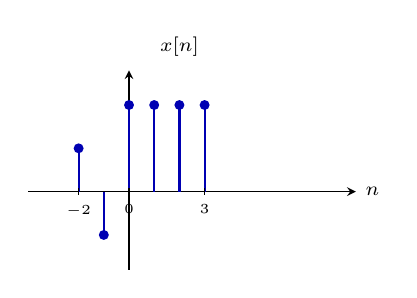
\begin{tikzpicture}[x=0.32cm,y=1.1cm,>=stealth]
  \draw[->] (-4,0) -- (9,0) node[right,font=\scriptsize] {$n$};
  \draw[->] (0,-0.9) -- (0,1.4);
  \stem{-2}{0.5} \stem{-1}{-0.5} \stem{0}{1} \stem{1}{1} \stem{2}{1} \stem{3}{1}
  \foreach \k in {-2,-1,0,1,2,3} { \node[below,font=\tiny] at (\k,-0.02) {};}
  \foreach \k in {-2,0,3} { \draw (\k,0.04)--(\k,-0.04) node[below,font=\tiny] {$\k$}; }
  \node[font=\scriptsize,anchor=south] at (2,1.45) {$x[n]$};
\end{tikzpicture}
\end{minipage}
\begin{minipage}{0.32\textwidth}\centering
\begin{tikzpicture}[x=0.32cm,y=1.1cm,>=stealth]
  \draw[->] (-4,0) -- (9,0) node[right,font=\scriptsize] {$n$};
  \draw[->] (0,-0.9) -- (0,1.4);
  \stem{1}{0.5} \stem{2}{-0.5} \stem{3}{1} \stem{4}{1} \stem{5}{1} \stem{6}{1}
  \foreach \k in {1,3,6} { \draw (\k,0.04)--(\k,-0.04) node[below,font=\tiny] {$\k$}; }
  \node[font=\scriptsize,anchor=south] at (3.5,1.45) {$x[n-3]$：右移 3};
\end{tikzpicture}
\end{minipage}
\begin{minipage}{0.32\textwidth}\centering
\begin{tikzpicture}[x=0.32cm,y=1.1cm,>=stealth]
  \draw[->] (-4,0) -- (9,0) node[right,font=\scriptsize] {$n$};
  \draw[->] (0,-0.9) -- (0,1.4);
  \stem{1}{1} \stem{2}{1} \stem{3}{1} \stem{4}{1} \stem{5}{-0.5} \stem{6}{0.5}
  \foreach \k in {1,4,6} { \draw (\k,0.04)--(\k,-0.04) node[below,font=\tiny] {$\k$}; }
  \node[font=\scriptsize,anchor=south] at (3.5,1.45) {$x[4-n]$：翻转再右移 4};
\end{tikzpicture}
\end{minipage}
\caption{离散信号的自变量变换。数据来自黑板：$x[n]$ 在 $n=-2,-1$ 处是 $\tfrac12,-\tfrac12$，在 $n=0,1,2,3$ 处是 $1$。}
\end{figure}

%==================================================================
\section{有了变换的概念，再看熟悉的信号}
老师说：脑子里有了「信号翻转过来翻转过去、放大缩小、移来移去」的概念之后，对信号的看法会不一样。下面是他举的几个例子。

\subsection{$\Sa(\omega t)$ 与 $\dfrac{\sin\omega t}{t}$}
已知 $\Sa(t)=\dfrac{\sin t}{t}$，画 $\Sa(\omega t)=\dfrac{\sin\omega t}{\omega t}$（$\omega>0$）。只用第三条口诀：系数是 $\omega$，$\omega>1$ 就压缩 $\omega$ 倍。原来的零点 $\pm\pi,\pm2\pi,\dots$ 变成 $\pm\dfrac{\pi}{\omega},\pm\dfrac{2\pi}{\omega},\dots$，峰高仍是 $1$。

老师接着说：前一节课让大家画的是 $\dfrac{\sin\omega t}{t}$，这个式子就是 $\omega\cdot\Sa(\omega t)$，所以只要把 $\Sa(\omega t)$ 再\textbf{乘一个 $\omega$}，峰高就是 $\omega$。这与上一份笔记里「峰高 $\omega$，零点 $\pm k\pi/\omega$」的结论一致。

\subsection{第五章的例子：$X(\omega/T)$}
老师说第五章会碰到一个标准的例子：$X(\omega)$ 是一个带限信号（band-limited signal，只在 $[-\omega_0,\omega_0]$ 上有值，其他地方为 $0$），峰值（$\omega=0$ 处）为 $E$。问：$X\bigl(\tfrac{\omega}{T}\bigr)$ 是什么形状？答案：\textbf{峰值仍是 $E$}，两个端点从 $\pm\omega_0$ 变成 $\pm T\omega_0$。这就是第三条口诀：系数 $\tfrac1T$，$T>1$ 时系数小于 $1$，是拉伸。\emph{（课堂口述把 $X(\omega/T)$ 听成了「$X\omega$ 除以 $T$」，黑板上写的是 $X(\frac{\omega}{T})$，所以我按黑板写。黑板图没有写 $T$ 的具体值。）}

\begin{figure}[H]
\centering
\begin{tikzpicture}[x=0.42cm,y=0.8cm,>=stealth]
  % 左：X(omega)
  \draw[->] (-4,0) -- (4.4,0) node[right,font=\scriptsize] {$\omega$};
  \draw[->] (0,-0.2) -- (0,2.8);
  \draw[very thick,blue!70!black,domain=-2:2,samples=60] plot (\x,{2*(1-(\x/2)^2)});
  \node[left,font=\scriptsize] at (0,2) {$E$};
  \node[below,font=\scriptsize] at (-2,0) {$-\omega_0$};
  \node[below,font=\scriptsize] at (2,0) {$\omega_0$};
  \node[font=\small] at (0,3.2) {$X(\omega)$};
  % 右：X(omega/T), 取 T=2
  \begin{scope}[xshift=7.2cm]
    \draw[->] (-6.4,0) -- (6.8,0) node[right,font=\scriptsize] {$\omega$};
    \draw[->] (0,-0.2) -- (0,2.8);
    \draw[very thick,red!70!black,domain=-4:4,samples=80] plot (\x,{2*(1-(\x/4)^2)});
    \node[left,font=\scriptsize] at (0,2) {$E$};
    \node[below,font=\scriptsize] at (-4,0) {$-T\omega_0$};
    \node[below,font=\scriptsize] at (4,0) {$T\omega_0$};
    \node[font=\small] at (0,3.2) {$X(\omega/T)$（图中取 $T=2$）};
  \end{scope}
\end{tikzpicture}
\caption{$X(\omega/T)$ 是 $X(\omega)$ 沿 $\omega$ 轴拉伸 $T$ 倍：峰值不变，宽度变成 $T$ 倍。左边的钟形只是示意，黑板上的具体形状同为一个拱形。}
\end{figure}

\subsection{用阶跃函数平移、做减法，表示各种「窗」}
\begin{enumerate}
\item $u(t-t_0)$：阶跃函数 $u(t)$ 的自变量减 $t_0$，\textbf{减号右移 $t_0$}：从 $t=t_0$ 开始等于 $1$。
\item 方波 $g(t)$：在 $0<t<t_0$ 上为 $1$，其他地方为 $0$。老师的写法：
\[
g(t)=u(t)-u(t-t_0).
\]
理由：$u(t)$ 从 $0$ 开始是 $1$，$u(t-t_0)$ 从 $t_0$ 开始是 $1$，两个相减：$t<0$ 时都是 $0$，$t>t_0$ 时是 $1-1=0$，只在 $0<t<t_0$ 一段 $1-0=1$。
\item 请大家画 $u(t+3)-u(t-3)$：加号左移 $3$，从 $t=-3$ 开始是 $1$；减号右移 $3$，从 $t=3$ 开始是 $1$；相减后 \textbf{在 $-3<t<3$ 上等于 $1$}，其他为 $0$。老师说这类题考察的核心就是「加号左移、减号右移」熟不熟。
\end{enumerate}

\begin{figure}[H]
\centering
\begin{minipage}{0.32\textwidth}\centering
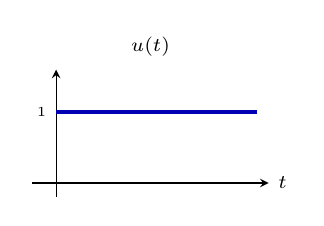
\begin{tikzpicture}[x=0.3cm,y=0.9cm,>=stealth]
  \draw[->] (-1,0) -- (9,0) node[right,font=\scriptsize] {$t$};
  \draw[->] (0,-0.2) -- (0,1.6);
  \draw[very thick,blue!70!black] (0,1) -- (8.5,1);
  \node[left,font=\tiny] at (0,1) {$1$};
  \node[font=\scriptsize,anchor=south] at (4,1.65) {$u(t)$};
\end{tikzpicture}
\end{minipage}
\begin{minipage}{0.32\textwidth}\centering
\begin{tikzpicture}[x=0.3cm,y=0.9cm,>=stealth]
  \draw[->] (-1,0) -- (9,0) node[right,font=\scriptsize] {$t$};
  \draw[->] (0,-0.2) -- (0,1.6);
  \draw[very thick,blue!70!black] (4,1) -- (8.5,1);
  \draw (4,0.05)--(4,-0.05) node[below,font=\tiny] {$t_0$};
  \node[font=\scriptsize,anchor=south] at (4,1.65) {$u(t-t_0)$：右移 $t_0$};
\end{tikzpicture}
\end{minipage}
\begin{minipage}{0.32\textwidth}\centering
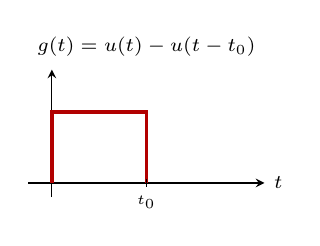
\begin{tikzpicture}[x=0.3cm,y=0.9cm,>=stealth]
  \draw[->] (-1,0) -- (9,0) node[right,font=\scriptsize] {$t$};
  \draw[->] (0,-0.2) -- (0,1.6);
  \draw[very thick,red!70!black] (0,0) -- (0,1) -- (4,1) -- (4,0);
  \draw (4,0.05)--(4,-0.05) node[below,font=\tiny] {$t_0$};
  \node[font=\scriptsize,anchor=south] at (4,1.65) {$g(t)=u(t)-u(t-t_0)$};
\end{tikzpicture}
\end{minipage}
\caption{用两个阶跃相减得到方波：$g(t)=u(t)-u(t-t_0)$。}
\end{figure}

\begin{figure}[H]
\centering
\begin{minipage}{0.32\textwidth}\centering
\begin{tikzpicture}[x=0.3cm,y=0.9cm,>=stealth]
  \draw[->] (-8,0) -- (8,0) node[right,font=\scriptsize] {$t$};
  \draw[->] (0,-0.2) -- (0,1.6);
  \draw[very thick,blue!70!black] (-3,1) -- (7.5,1);
  \draw (-3,0.05)--(-3,-0.05) node[below,font=\tiny] {$-3$};
  \node[font=\scriptsize,anchor=south] at (0,1.65) {$u(t+3)$：左移 3};
\end{tikzpicture}
\end{minipage}
\begin{minipage}{0.32\textwidth}\centering
\begin{tikzpicture}[x=0.3cm,y=0.9cm,>=stealth]
  \draw[->] (-8,0) -- (8,0) node[right,font=\scriptsize] {$t$};
  \draw[->] (0,-0.2) -- (0,1.6);
  \draw[very thick,blue!70!black] (3,1) -- (7.5,1);
  \draw (3,0.05)--(3,-0.05) node[below,font=\tiny] {$3$};
  \node[font=\scriptsize,anchor=south] at (0,1.65) {$u(t-3)$：右移 3};
\end{tikzpicture}
\end{minipage}
\begin{minipage}{0.32\textwidth}\centering
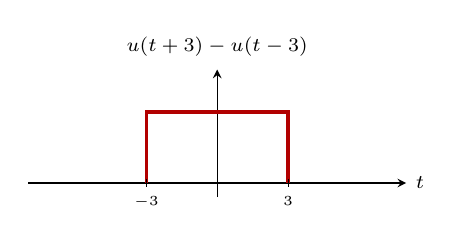
\begin{tikzpicture}[x=0.3cm,y=0.9cm,>=stealth]
  \draw[->] (-8,0) -- (8,0) node[right,font=\scriptsize] {$t$};
  \draw[->] (0,-0.2) -- (0,1.6);
  \draw[very thick,red!70!black] (-3,0) -- (-3,1) -- (3,1) -- (3,0);
  \draw (-3,0.05)--(-3,-0.05) node[below,font=\tiny] {$-3$};
  \draw (3,0.05)--(3,-0.05) node[below,font=\tiny] {$3$};
  \node[font=\scriptsize,anchor=south] at (0,1.65) {$u(t+3)-u(t-3)$};
\end{tikzpicture}
\end{minipage}
\caption{$u(t+3)-u(t-3)$ 在 $-3<t<3$ 上等于 $1$。}
\end{figure}

\subsubsection*{离散的版本}
\begin{enumerate}
\item $g_N[n]$：在 $n=0,1,\dots,N-1$ 上为 $1$，其余为 $0$。写法：$g_N[n]=u[n]-u[n-N]$。理由：$u[n]$ 从 $0$ 开始是 $1$，$u[n-N]$ 从 $N$ 开始是 $1$，相减后只在 $0\le n\le N-1$ 上是 $1$。
\item 请画 $u[n+2]-u[n-3]$：$u[n+2]$ 从 $n=-2$ 开始是 $1$，$u[n-3]$ 从 $n=3$ 开始是 $1$，相减后\textbf{在 $n=-2,-1,0,1,2$（共 5 个点）上是 $1$，其余为 $0$}。
\end{enumerate}
老师特别提醒：离散的这类题比连续的\textbf{稍微烧脑}，难点是「\textbf{在边界处哪里开始等于零}」要算清楚：右边在 $n=3$ 处，两个阶跃都是 $1$，相减等于 $0$，所以右端点是 $n=2$ 而不是 $n=3$。
\emph{（转写里老师口述的区间听起来是「负二到二」，板书我没有找到这一道题的画面，上面的结果是我按定义算的。）}

\begin{figure}[H]
\centering
\begin{minipage}{0.48\textwidth}\centering
\begin{tikzpicture}[x=0.38cm,y=0.9cm,>=stealth]
  \draw[->] (-1,0) -- (10,0) node[right,font=\scriptsize] {$n$};
  \draw[->] (0,-0.2) -- (0,1.5);
  \foreach \k in {0,1,2,3} { \stem{\k}{1} }
  \foreach \k in {-1} { \stemzero{\k} }
  \foreach \k in {4,5,6} { \stemzero{\k} }
  \foreach \k in {0,3} { \draw (\k,0.04)--(\k,-0.04) node[below,font=\tiny] {$\k$}; }
  \node[below,font=\tiny] at (4,-0.04) {$N$};
  \node[font=\scriptsize,anchor=south] at (4,1.55) {$g_N[n]=u[n]-u[n-N]$（图中 $N=4$）};
\end{tikzpicture}
\end{minipage}
\begin{minipage}{0.48\textwidth}\centering
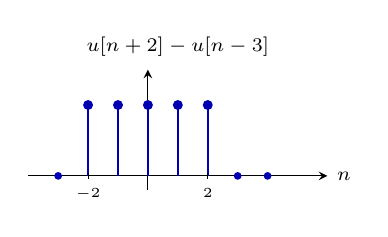
\begin{tikzpicture}[x=0.38cm,y=0.9cm,>=stealth]
  \draw[->] (-4,0) -- (6,0) node[right,font=\scriptsize] {$n$};
  \draw[->] (0,-0.2) -- (0,1.5);
  \foreach \k in {-2,-1,0,1,2} { \stem{\k}{1} }
  \foreach \k in {-3,3,4} { \stemzero{\k} }
  \foreach \k in {-2,2} { \draw (\k,0.04)--(\k,-0.04) node[below,font=\tiny] {$\k$}; }
  \node[font=\scriptsize,anchor=south] at (1,1.55) {$u[n+2]-u[n-3]$};
\end{tikzpicture}
\end{minipage}
\caption{离散的「窗」：左，$g_N[n]$（$N=4$）；右，$u[n+2]-u[n-3]$ 在 $n=-2,\dots,2$ 上为 $1$。}
\end{figure}

\subsection{把序列写成冲激的和}
老师给的例子：$x[n]$ 在 $n=-2,-1,0,1,2$ 处分别是 $1,2,1,-1,-2$，其余为 $0$。问：能看出它等于下面这个式子吗？
\[
x[n]=\delta[n+2]+2\,\delta[n+1]+\delta[n]-\delta[n-1]-2\,\delta[n-2].
\]
老师的解释（用的还是那两句口诀）：
\begin{itemize}[nosep]
\item $\delta[n]$ 只在 $n=0$ 处是 $1$；
\item $\delta[n+2]$：加号左移 $2$，在 $n=-2$ 处是 $1$，所以第一项刚好对应 $x[-2]=1$；
\item $\delta[n+1]$ 在 $n=-1$ 处是 $1$，但 $x[-1]=2$，所以要乘 $2$：$2\delta[n+1]$；
\item $\delta[n-1]$：减号右移 $1$，在 $n=1$ 处是 $1$，而 $x[1]=-1$，所以乘 $-1$；
\item 同理 $-2\,\delta[n-2]$ 对应 $x[2]=-2$。
\end{itemize}
老师说：考试时很多同学看到这样的序列「不知所措」，其实你应该马上反应到：它就是若干个平移过的单位脉冲，每一个按对应的值加权，再加起来。

\begin{figure}[H]
\centering
\begin{minipage}{0.32\textwidth}\centering
\begin{tikzpicture}[x=0.34cm,y=0.5cm,>=stealth]
  \draw[->] (-4,0) -- (4.5,0) node[right,font=\scriptsize] {$n$};
  \draw[->] (0,-2.8) -- (0,3);
  \stem{-2}{1} \stem{-1}{2} \stem{0}{1} \stem{1}{-1} \stem{2}{-2}
  \foreach \k in {-2,-1,1,2} { \node[font=\tiny,above] at (\k,0) {}; }
  \node[font=\scriptsize,anchor=south] at (0,3.1) {$x[n]$};
\end{tikzpicture}
\end{minipage}
\begin{minipage}{0.32\textwidth}\centering
\begin{tikzpicture}[x=0.34cm,y=0.5cm,>=stealth]
  \draw[->] (-4,0) -- (4.5,0) node[right,font=\scriptsize] {$n$};
  \draw[->] (0,-2.8) -- (0,3);
  \stem{-2}{1}
  \node[font=\scriptsize,anchor=south] at (0,3.1) {$\delta[n+2]$};
\end{tikzpicture}
\end{minipage}
\begin{minipage}{0.32\textwidth}\centering
\begin{tikzpicture}[x=0.34cm,y=0.5cm,>=stealth]
  \draw[->] (-4,0) -- (4.5,0) node[right,font=\scriptsize] {$n$};
  \draw[->] (0,-2.8) -- (0,3);
  \stem{-1}{2}
  \node[font=\scriptsize,anchor=south] at (0,3.1) {$2\delta[n+1]$};
\end{tikzpicture}
\end{minipage}

\medskip
\begin{minipage}{0.32\textwidth}\centering
\begin{tikzpicture}[x=0.34cm,y=0.5cm,>=stealth]
  \draw[->] (-4,0) -- (4.5,0) node[right,font=\scriptsize] {$n$};
  \draw[->] (0,-2.8) -- (0,3);
  \stem{0}{1}
  \node[font=\scriptsize,anchor=south] at (0,3.1) {$\delta[n]$};
\end{tikzpicture}
\end{minipage}
\begin{minipage}{0.32\textwidth}\centering
\begin{tikzpicture}[x=0.34cm,y=0.5cm,>=stealth]
  \draw[->] (-4,0) -- (4.5,0) node[right,font=\scriptsize] {$n$};
  \draw[->] (0,-2.8) -- (0,3);
  \stem{1}{-1}
  \node[font=\scriptsize,anchor=south] at (0,3.1) {$-\delta[n-1]$};
\end{tikzpicture}
\end{minipage}
\begin{minipage}{0.32\textwidth}\centering
\begin{tikzpicture}[x=0.34cm,y=0.5cm,>=stealth]
  \draw[->] (-4,0) -- (4.5,0) node[right,font=\scriptsize] {$n$};
  \draw[->] (0,-2.8) -- (0,3);
  \stem{2}{-2}
  \node[font=\scriptsize,anchor=south] at (0,3.1) {$-2\delta[n-2]$};
\end{tikzpicture}
\end{minipage}
\caption{把 $x[n]$ 拆成五个平移并加权的单位脉冲：五个分量相加就是左上角的 $x[n]$。（数据来自黑板：$x[-2..2]=1,2,1,-1,-2$。）}
\end{figure}

\subsubsection*{一个著名的公式（书第 45 页，式 2-28）}
\begin{remember}
\[
x[n]=\sum_{k=-\infty}^{+\infty}x[k]\,\delta[n-k]
\]
\end{remember}
老师先写在黑板上，说「你通过做刚才的题，对这个公式会觉得它好像是对的」，并解释：
\begin{itemize}[nosep]
\item $x[k]$ 是 $x[n]$ 在 $n=k$ 处的值（一个数）；
\item $\delta[n-k]$ 是在 $n=k$ 处为 $1$、其他处为 $0$ 的信号；
\item 两者相乘，得到「只在 $n=k$ 处等于 $x[k]$，其余处为 $0$」的信号；
\item 对每一个不同的 $k$ 都这样做，再全部加起来，每个位置 $n$ 上都取到了正确的值。
\end{itemize}
老师说这个公式「稍微有点抽象」，第二章还会再讲；他认为只要脑子里有「一来一去」（移来移去）的概念，这个公式应该是能理解的。上面例子里的五项相加，就是它的一个具体实例（只有 $k=-2,\dots,2$ 这五项非零）。

%==================================================================
\section{本节要记住的清单}
\begin{enumerate}[nosep]
\item 四句口诀：\textbf{化成标准形式；前有负号翻转；系数绝对值大于 $1$ 压缩、小于 $1$ 拉伸；加号左移、减号右移}。
\item 标准形式：把 $t$ 前面的系数提出去，$x(at+b)=x\bigl(a(t+\tfrac ba)\bigr)$，平移量是 $b/a$。
\item 做法顺序：翻转 $\to$ 压缩或拉伸 $\to$ 平移。验算：取一两个关键点代入。
\item 反过来的题（已知变换后的，求原来的）：先把「要求的」写成关于已知函数的自变量变换，再套口诀。
\item 离散：$n$ 的系数基本是 $\pm1$，只用「翻转」和「平移」。
\item 窗函数：$u(t-t_0)$ 右移；$u(t)-u(t-t_0)$ 是 $(0,t_0)$ 上的方波；$u[n]-u[n-N]$ 是 $0\le n\le N-1$ 上的窗。
\item $x[n]=\sum_kx[k]\,\delta[n-k]$：序列等于平移并加权的单位脉冲之和。
\end{enumerate}

\end{document}
